\chapter{Approach \& Results}\label{chap:approach_results}

This chapter presents the main body of work resultant of the study performed for this dissertation, and it is divided in two main parts. The first one is related to research design and it starts by describing how the current design of the \emph{escolinhas.pt} platform was performed and which tools were used to perform the analysis, and how the variability needs for each one of the areas described in \ref{sec:case-study_areas} were identified. The second part describes the development process of each one of the case-study areas: Roles, Social Network and Document Editor. For each one of these areas, it will present the current design and variability requirements. Based on these informations, candidate patterns will be presented, as well as the chosen patterns used to solve the problem and the rationale behind it, outlining why certain patterns were discarded. Then, implementation details will follow, concluding each section with an analysis of the impact each solution had, as well as some results (where applicable).

\section{Research Design}\label{sec:research_design}

The first step taken in order to identify potential problems was to study its current design. This step led to the identification of several points that negatively impacted the variability of the application. After the identification of these points, variability requirements were gathered, so that small, functional prototypes could be built and their impact analyzed within the platform.

\subsection{Current Design Analysis}\label{sec:current_design_analysis}

A thorough analysis of the current design of the application was the first step taken, in order to identify potential problems within the platform. This study was conducted using a series of tools\footnote{Rubymine 2.0~\cite{rubymine} and Rails ERD~\cite{rails_erd}} that, unfortunately (at the time of writing), proved unsuccessful in extracting an \emph{Entity Relationship Diagram} from the code of the application --- either they did not work with the current versions of Ruby/Rails used by the platform (Rails ERD) or generated an inaccurate graph (Rubymine 2.0). As such, another approach was taken: the product owner of the platform was queried on what he felt were the variability ``hotspots'' of the application: this narrowed the scope of the current design analysis, allowing to focus on three different areas, as stated in~\ref{sec:case-study_areas}. These areas were then manually studied --- by analyzing the current database schema, as well as the Model (MVC) source files --- in order to extract the \emph{Entity Relationship Diagrams} relative to each one --- shown ahead on \ref{sec:fa_roles_variability_requirements}, \ref{sec:fa_social_network} and \ref{sec:fa_documents} --- which allowed analyzing each one as independently as possible, so that the applied design patterns (if any) would emerge --- making the task of pinpointing exactly what was wrong with each approach much easier.

\subsection{Variability Analysis}\label{sec:variability_analysis}

Each one of the areas --- Roles, Social Network and the Document Editor --- referred in \ref{sec:case-study_areas} was then studied in order to determine their variability requirements, and to which degree this variability should exist: developer, system administrator, or even end-user. These requirements were defined by the carefully considering the opinions from the users of the platform, the product owner and the main developers. These requirements were then used to determine which design patterns would be more appropriate to achieve the problems posed by each of the areas, and why.

\subsection{Implementation \& Impact Analysis}

For each one the three focus areas, functional prototypes were developed, either directly on top of the platform (Social Network, \ref{sec:fa_social_network}, and User Roles, \ref{sec:fa_roles}) or as an independent proof-of-concept application (Document Editor, \ref{sec:fa_documents}), that, as soon as possible, will be integrated into the main platform. These prototypes, however simplistic (and not yet in production), will be able to validate the research and decisions made throughout the next sections. All of the prototypes are implemented using Ruby 1.9.1 and Rails 2.3.9, as used in the production and development environments of \emph{escolinhas.pt}.

The impact analysis for each of these areas will be made in two different fronts: variability and performance. Variability impact analysis will be concerned with the increase in flexibility/configurability of a certain component, and how it measures to the objectives established beforehand. Performance analysis will (if applicable) examine the how much more (or less) performant each one of the implementations is, compared to the previous solutions.

After studying the current design of the application and collecting the necessary requirements, the development phase took place: the major variability requirements were outlined, and a set of design patterns carefully considered, with their benefits and disadvantages weighed in order to correctly choose the most appropriate solution. Finally, proof-of-concept prototypes were built so that the choice of patterns could be validated and the impact resultant from the implementations measured.

\subsection{User Roles}\label{sec:fa_roles}

Roles play a very important part in any application: by attaching them to users, they allow the application to authenticate and authorize users based on their roles. If an application has a strong tendency to evolve, so do its roles and authorization sets. This section describes the work involved in making the current system of roles used in \emph{escolinhas.pt} as adaptable as possible.

\subsubsection{Variability Requirements}\label{sec:fa_roles_variability_requirements}

Authorization is one of the most sensitive areas of any closed software system: it ensures everyone does only what it should in order to guarantee everything works as expected. In a constantly evolving system, the accesses granted by user roles have a tendency to shift and evolve alongside the application --- either because of new features or a new type of user is required in the system to perform specific tasks. In the context of \emph{escolinhas.pt} this problem ties itself with the ACL used: because of the diversity of roles (Fig.~\ref{fig:user_roles_current}) and the three different usage plans, a lot of different rules are applied to determine if a user can or can not perform certain actions; allied to the growing number of features of the platform, this means that the authorization scheme has to be as flexible as possible to ensure minimal overhead when determining new types of permission sets.

\begin{figure}[h]
  \centering
  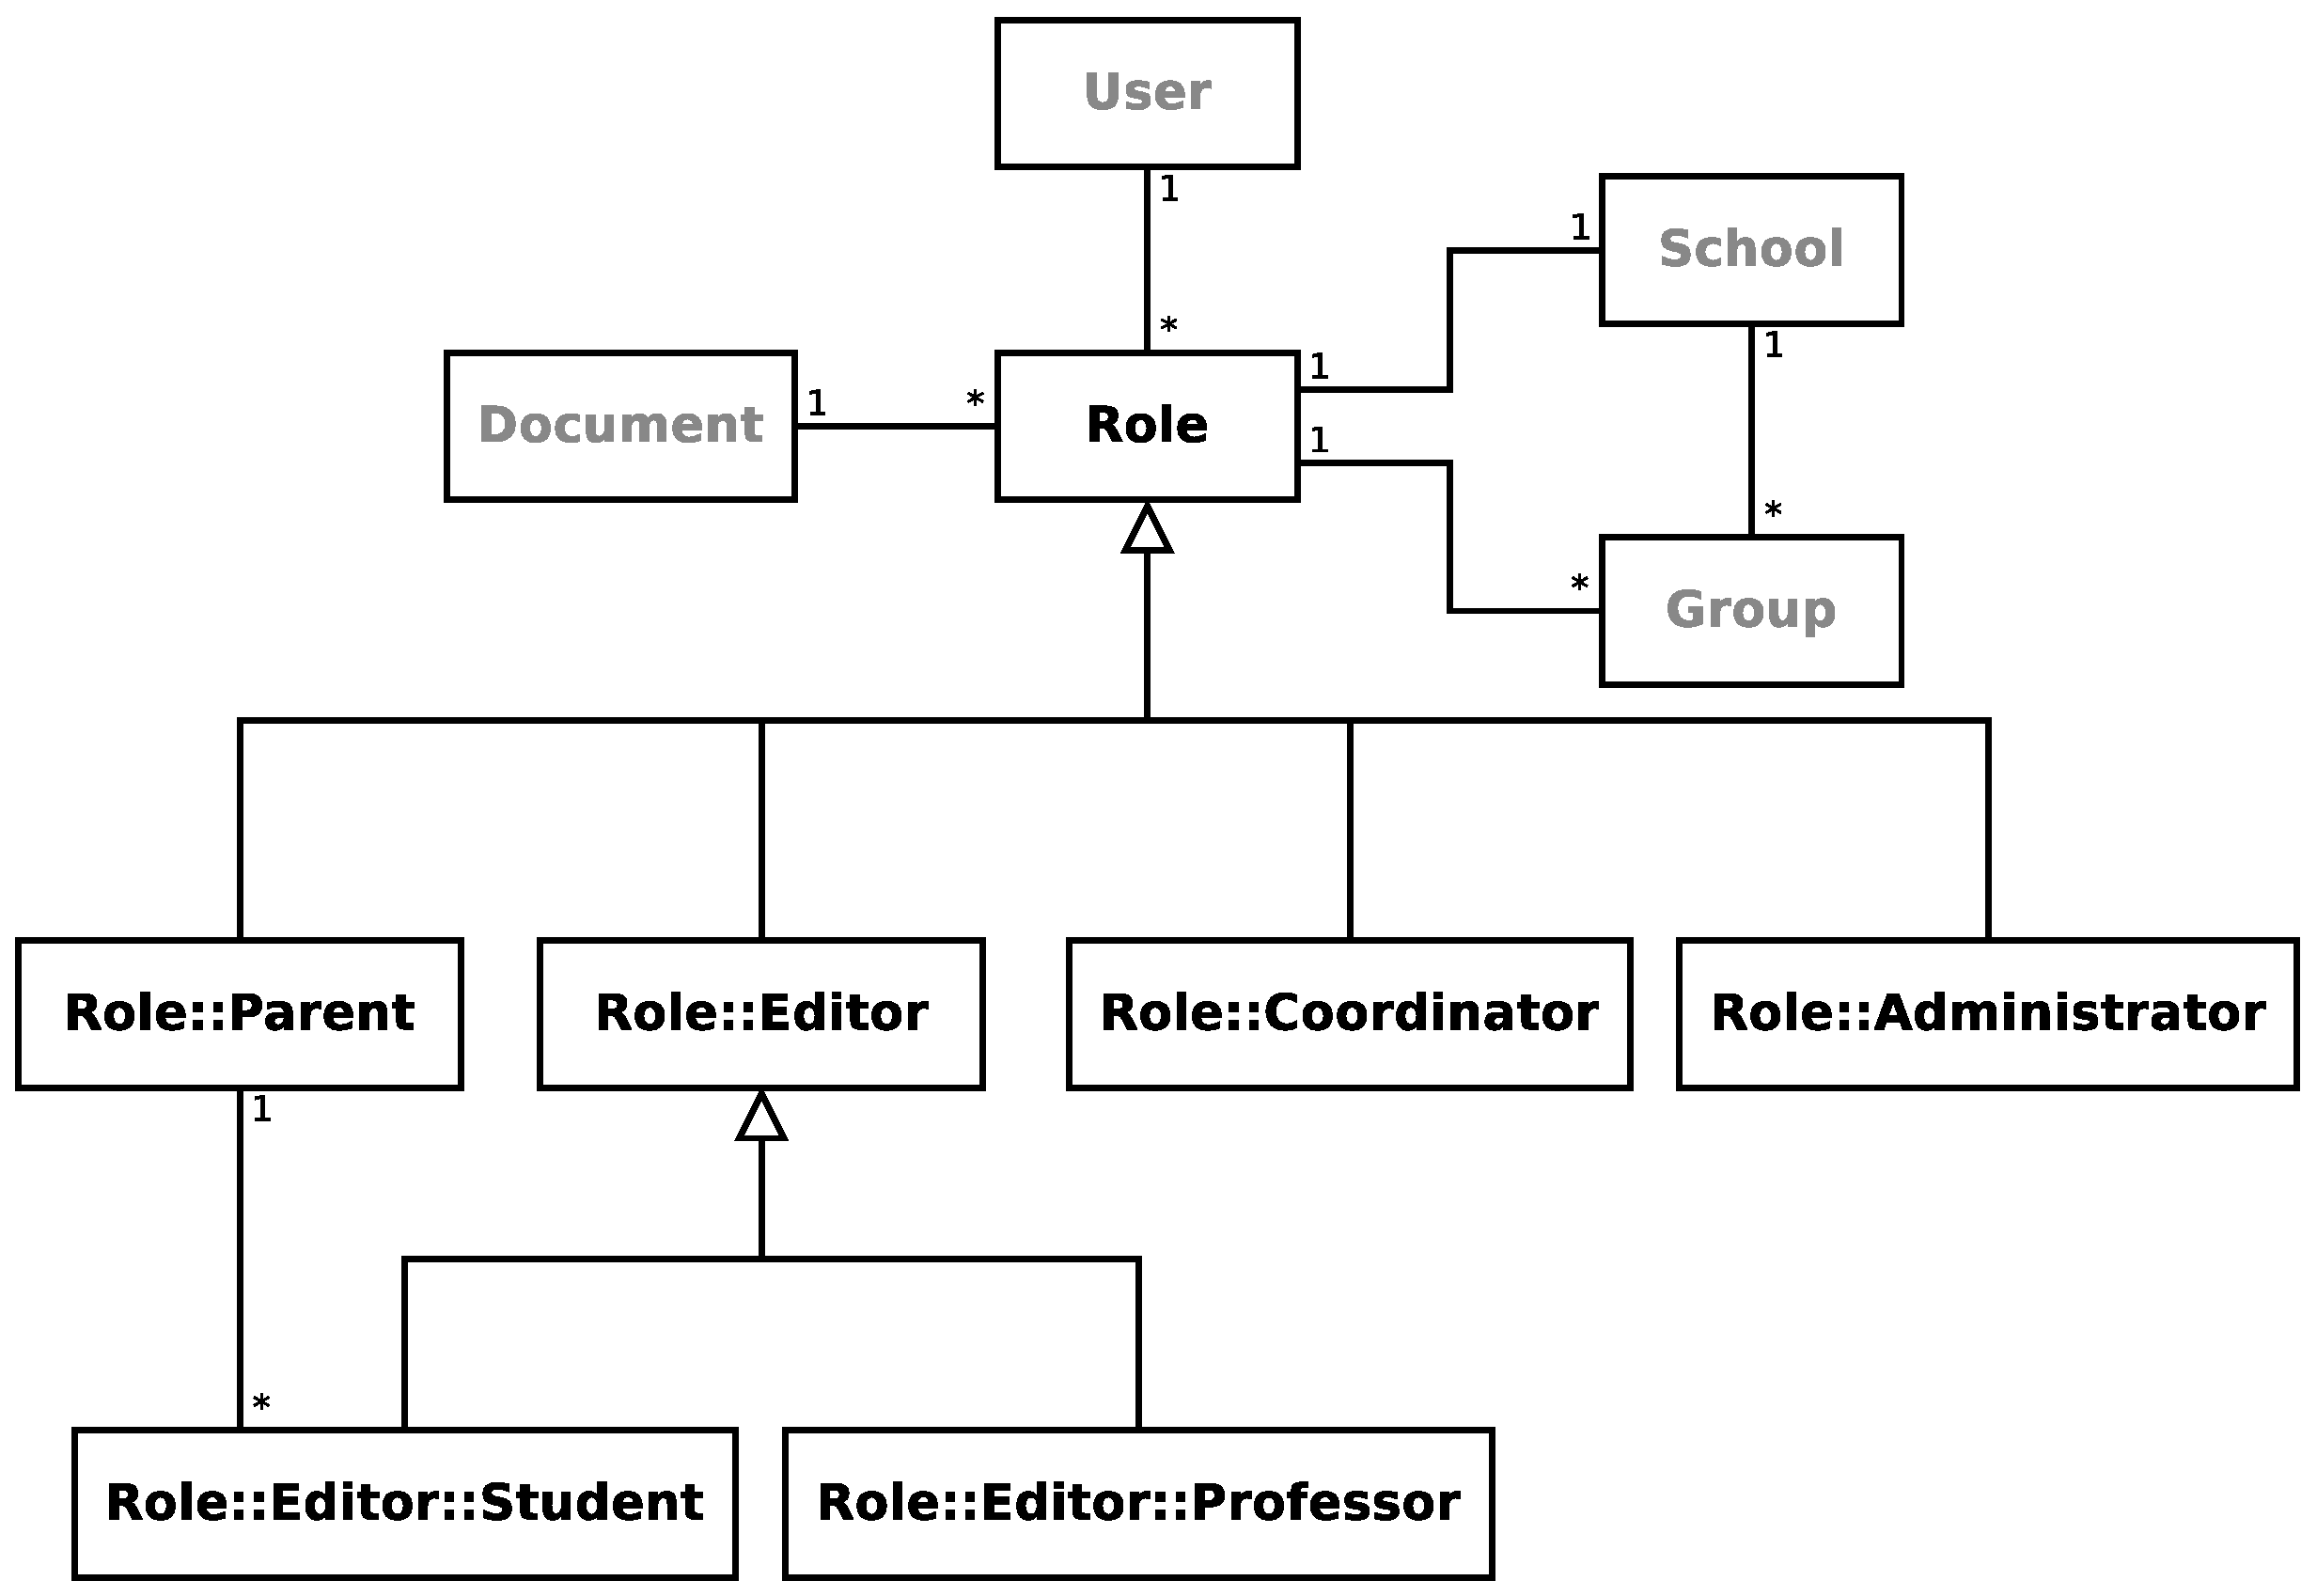
\includegraphics[width=130mm]{user_roles_current}
  \caption{Current User Roles Model}
  \label{fig:user_roles_current}
\end{figure}

\subsubsection{Candidate Patterns}\label{sec:fa_roles_candidate_patterns}

The current logic on roles and users states that a user may be a professor, a student, a parent, a coordinator (in which case it also has a professor role associated), or an administrator. Of these five different types of roles, only two of them are allowed editing privileges, which means that only students and professors have to ability to create and edit documents, which leads to an unnecessary level of complexity. If, for example, it was necessary to have a parent with editing privileges, a new Role, descendant of Role::Editor, would have to be created just for that user.

An obvious solution to this problem would be to tie a ``traditional'' \textsc{Access Control List} (as described in \cite{acls}) to the roles actually in use: this would allow to fine-tune each one of the users permissions and authorization sets while maintaining the codebase clean --- however, the logic surrounding authorization schemas and user roles is built around the \emph{CanCan} Ruby gem \cite{cancan}, which authorizes an user based on his or her roles, while keeping the necessary logic to a minimum.

As such, the usage of a full-fledged ACL is unnecessary. As \emph{CanCan} rules are written in Ruby and are based on the AR engine used by Rails, \emph{CanCan} is capable of handling authorizations based either on Models (MVC) or \emph{instances} of these Models. The application of an ACL to define user permissions would allow a fine-grained control over the actions of every individual --- instances of \emph{User} Model --- on the system. However, the cases when this kind of control is necessary are rare, which would mean that the increase in complexity brought with the usage of an ACL would not be surpassed by its usefulness: it would be necessary to rewrite every rule already defined within \emph{CanCan} and then associate each user on the system with a specific set of rules, instead of maintaining the current setup and writing a few (rare) exceptions for the users the system administrator saw fit.

\subsubsection{Chosen Patterns \& Rationale}\label{sec:fa_roles_chosen_patterns_rationale}

As the implementation of an ACL was discarded in \ref{sec:fa_roles_candidate_patterns}, the best solution is to enhance the already present roles system: a flat Role hierarchy, as described in \cite{baumer_riehle_role_object} would allow for a more flexible authorization scheme, where a User could have one or more roles associated, depending on what actions he would be allowed to do, as shown on Fig.~\ref{fig:user_roles_conceptual}. This also makes the task of creating new roles with different authorization schemes much easier, as there is not a need to conform to any special hierarchy scheme: a new role simply means a new type of user. This clearly contrasts with the previous role's logic, where a multi-level hierarchy was in place.

\begin{figure}[H]
  \centering
  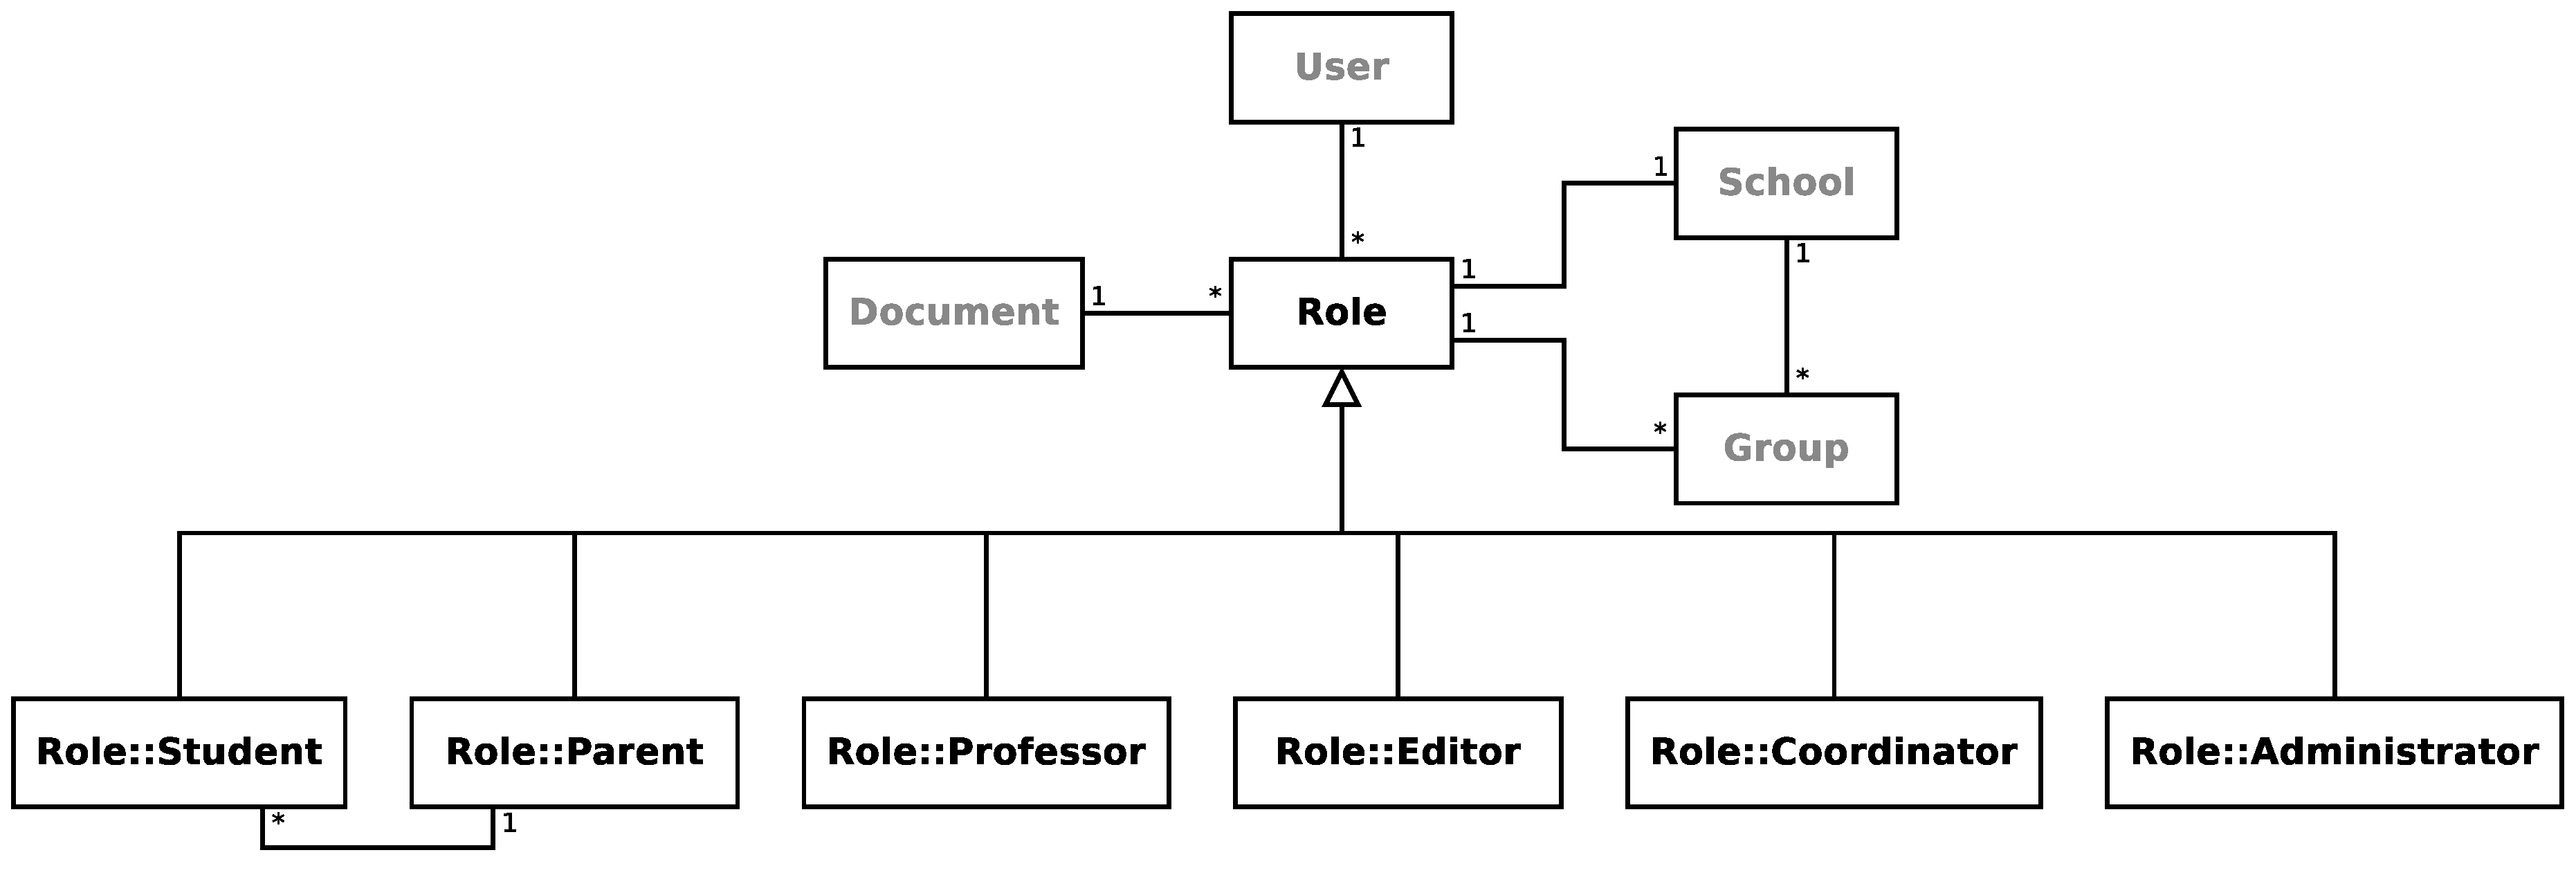
\includegraphics[width=160mm]{user_roles_conceptual}
  \caption{Conceptual User Roles Model}
  \label{fig:user_roles_conceptual}
\end{figure}

\subsubsection{Implementation}\label{sec:fa_roles_implementation}

The refactoring of the roles infrastructure was of very low impact, as codebase and database schema are regarded. The hierarchy of Role classes was flattened, keeping it at only two levels: a generic, non-instantiable class \emph{Role}, and all of its currently existent subclasses: \emph{Editor, Parent, Student, Professor, Coordinator} and \emph{Administrator}. Then, the existent rules were adapted to fit this new hierarchy. The last steps pertains to the modification of the current data to fit the new role organization, which entails analyzing each user current roles and performing the adequate substitutions from the previous roles schema. 

\subsubsection{Impact Analysis}\label{sec:fa_roles_impact_analysis}

The main issues related to the current Roles schema and consequent authorization strategies are caused by the difficulty to capture the constantly evolving necessities of different types of users. As the platform evolves, so do its users and their associated roles. If a new feature is added to the application, it is necessary to define the privileges each user type has over it. The flattening of the Roles hierarchy allows the representation of this Roles as separate, independent objects, allowing the different contexts they refer to be kept separate and also simplify the system configuration.

The usage of a \emph{matricial} ACL implementation, as discussed in \ref{sec:fa_roles_candidate_patterns} would simplify the configuration regarding the privileges of specific users --- allowing a system administrator to have full control over them. Ultimately, this means that the roles would play a very small part in authorization granting, serving only as pre-defined rule sets to be applied to new users.

The usage of a \emph{declarative} ACL (\emph{CanCan}) in conjunction with the \textsc{Role Object} pattern, leads to some important consequences: despite losing the ability to \emph{easily} control the specific set of rules of each user\footnotemark and increasing the difficulty of maintaining constraints between roles, it allows the independent evolution of each \emph{Role}, while making the task of defining their key abstractions regarding each role's position within the platform much more simple and concise.

\footnotetext{This ability  is not completely lost: if necessary, \emph{CanCan} can be used to define authorizations based on a User instance (a specific user)}

%The only relevant point of impact is related to variability. Albeit a low-impact modification, the refactoring of the Roles hierarchy allows for a much quicker role engineering process. This is because a Role now corresponds to a single set of rules, without any hindrance resulting from the previous rule hierarchy. The fact that a multitude of Roles can be associated with a single user allows for a much more wider range of authorizations schemes, as privileges originating from different Roles can be mixed to create unique privilege sets, adapting to a number of different needs.

%\ \\
%\textbf{FIXME: briefly explain how conflicting rules work}





\section{Social Network}\label{sec:fa_social_network}

The current design for the escolinhas.pt social network is dynamic in nature, and extracted from the relationships formed through the connections between users and their roles with schools, groups, and even another roles, as depicted in Fig.~\ref{fig:social_network_current}. This allows the construction of a network where all the connections can be inferred dynamically and where an user can be identified another through their connections: friends, classmates, parent--child, teacher--student, and so on. This network is used mainly in the internal messaging system (and, in a brief future, the instant messaging, or chat system) of \emph{escolinhas.pt}, which allows users to communicate with each other within the platform.

\begin{figure}[H]
  \centering
  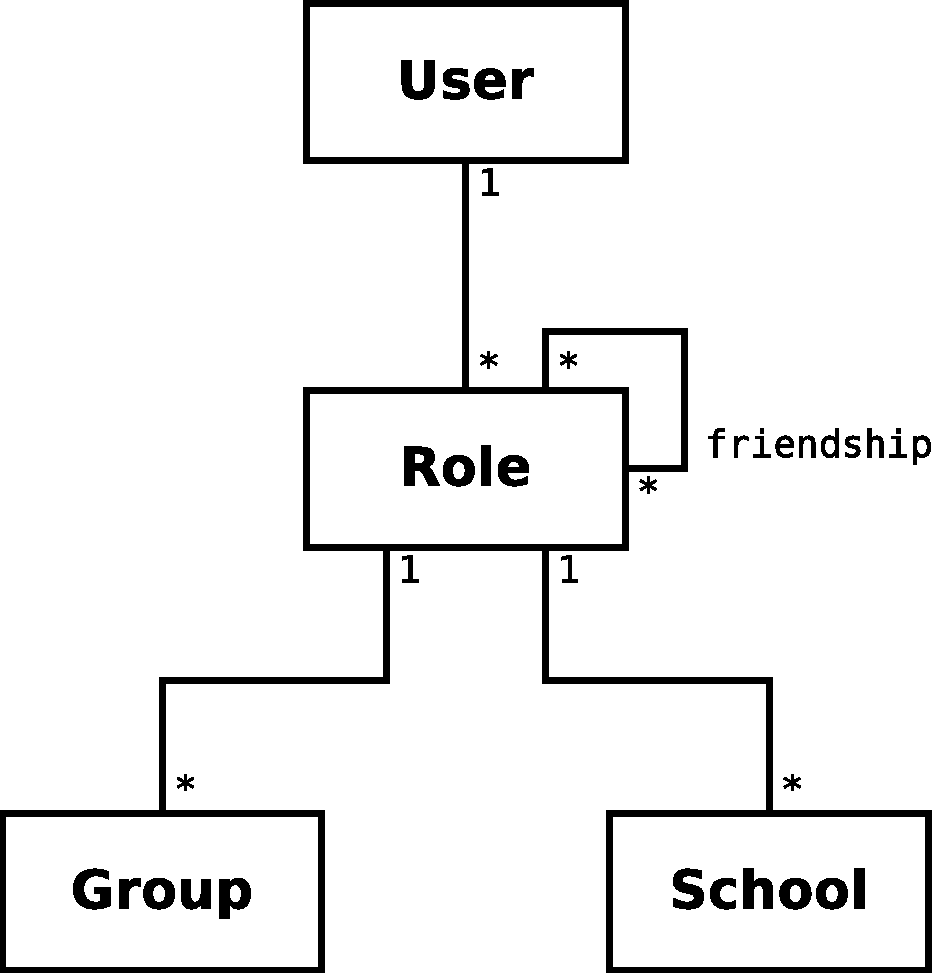
\includegraphics[width=65mm]{social_network_current.pdf}
  \caption{Current User Network Model}
  \label{fig:social_network_current}
\end{figure}

\subsection{Variability Requirements}\label{sec:fa_social_network_variability_requirements}

This model, however useful, offers a very small degree of variability. Due to the closed nature of the platform, there is a need to provide mechanisms able to fine-tune these connections in order to cater to each school specific needs. These mechanisms need to be available at the system administrator level, in order to easily manipulate these links without the need to pollute the application's codebase with hard-coded rules and without the need for redeployement.

\subsection{Candidate Patterns}\label{sec:fa_social_network_candidate_patterns}

Ideally, the user network would be described with a simple, self-referencing model, as shown in figure~\ref{fig:ideal_social_network_users}. This would allow the creation of static relationships between any two users that could be edited as needed. This would work great if all that was needed was to create realtionships between users. However, it is often necessary to create connections between users and other entities in the system, such as groups and schools. Thus, this simple model needs to be abstracted in order to connect any two entities present in the system, whichever they may be, as shown in Fig.~\ref{fig:ideal_social_network_things}.

\begin{figure}[H]
  \centering
  \subfloat[Users Network]{\label{fig:ideal_social_network_users}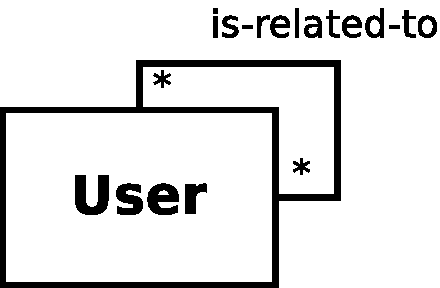
\includegraphics[width=25mm]{ideal_social_network_users}}
  \hspace{20mm}
  \subfloat[Entities Network]{\label{fig:ideal_social_network_things}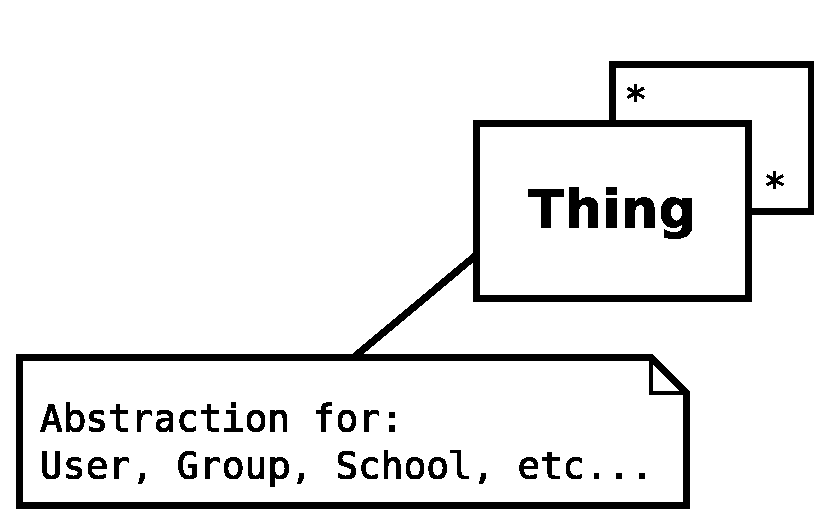
\includegraphics[width=55mm]{ideal_social_network_things}}
  \caption{Simplified Network Models}
  \label{fig:simplified_network_models}
\end{figure}

\subsection{Chosen Patterns \& Rationale}\label{sec:fa_social_network_chosen_patterns_rationale}

Despite solving the majority of the problem, the solutions described in \ref{sec:fa_social_network_candidate_patterns} are less than ideal, as they do not allow the identification of an user before another, because only a direct connection between two different entities is contemplated. As such, for this particular problem, it is necessary to be able to connect any two entities in the system, with an optional third entity to serve as hint as to how the original entities are connected. This problem can be solved by using the \textsc{Accountability} pattern (see \ref{sec:relationships_between_entities}) by Martin Fowler \cite{fowler_accountability}: it allows a bi-directional relationship between two entities (also known as \emph{parties}) while maintaining an AccountabilityType which can be used to store aditional data about the connection. As such, this AccountabilityType can be used to store an optional third party, responsible for identifying how the two other parties are connected --- effectivelly granting means to identify an user before an other, which is part of the original problem formulation (\ref{sec:fa_social_network}).

\subsection{Implementation}\label{sec:fa_social_network_implementation}

A variant of the \textsc{Accountability} design pattern was chosen (shown in Fig.~\ref{fig:social_network_conceptual}). This implementation follows the original description of the pattern by using all the usual entities present in the original \textsc{Accountability} pattern \cite{fowler_accountability} --- however, it denormalizes the AccountabilityType entity \emph{into} the Accountabilities themselves, by placing the AccountabilityType attributes (\verb!type!, \verb!through!, \verb!school_year!, \verb!active!) in the Accountability. Despite creating some data redundancy, this option provides a more performant implementation: as the Accountabilities table is to be constantly accessed, the decision to have the AccountabilityTypes in a separate table would lead to expensive \verb!JOIN! operations. This, in turn, would lead to a less than desirable performance and complexity.

\begin{figure}[H]
  \centering
  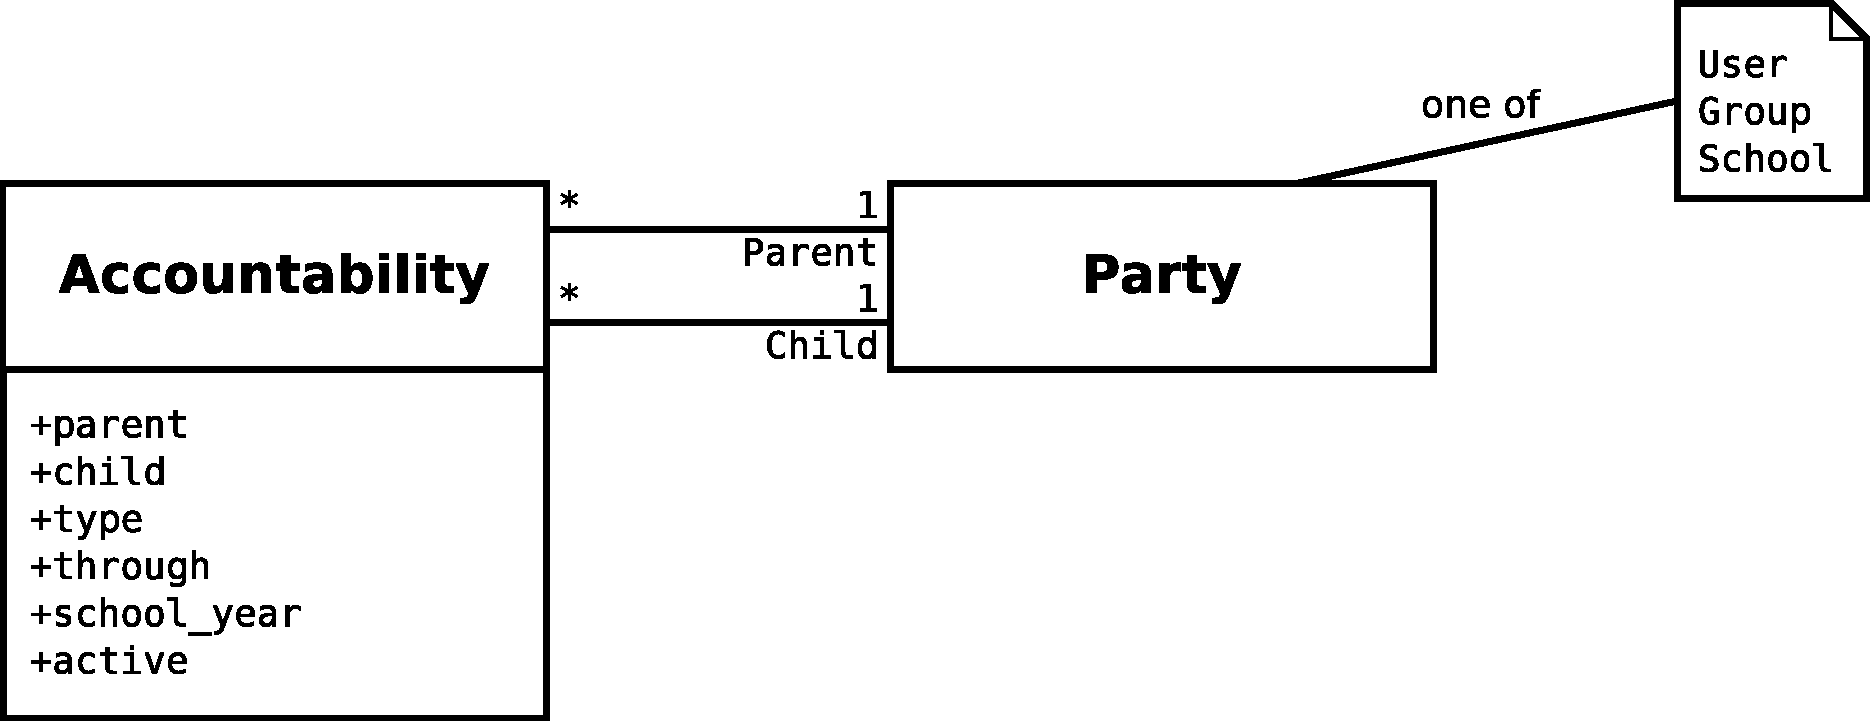
\includegraphics[width=115mm]{social_network_conceptual}
  \caption{Accountability Implementation for User Network}
  \label{fig:social_network_conceptual}
\end{figure}

A series of different AccountabilityTypes were created, in order to cater to a multitude of relationship types:

\begin{itemize}
  \item \textbf{group\_professor:} establishes a connection between a \emph{Group} and a \emph{Professor}, meaning that the user is one of the teacher of \emph{Group}
  \item \textbf{professor:} establishes a connection between two \emph{Users} --- a \emph{Professor} and a \emph{Student} --- creating a teacher-student relationship between them through whichever \emph{Group} they are related to
  \item \textbf{group\_student:} establishes a connection between a \emph{Group} and a \emph{Student}, meaning that the user is part of the \emph{Group} and taught by the \textbf{group\_professors} associated with the aforementioned \emph{Group}
  \item \textbf{school\_professor:} establishes a connection between a \emph{School} and a \emph{Professor}
  \item \textbf{school\_student:} establishes a connection between a \emph{School} and a \emph{Student}
  \item \textbf{parent:} establishes a parenthood relationship between two users
  \item \textbf{school\_coordinator:} dictates an \emph{User} is a coordinator (also known as an administrator) of a certain \emph{School}
  \item \textbf{colleague:} establishes a connection between two \emph{Users} --- either a \emph{Coordinator} or a \emph{Professor} --- through a \emph{School} they both work in
  \item \textbf{student:} establishes a relationship between a \emph{Coordinator} and a \emph{Student} through a \emph{School}
  \item \textbf{school\_parent:} establishes a relationship between a \emph{Coordinator} and a \emph{Parent} through a \emph{School}
  \item \textbf{friend:} establishes a connection between any two \emph{Users} of the system --- whichever their roles may be --- to indicate a friendship relation exists between them
\end{itemize}

% generated with http://truben.no/latex/table/
%\begin{table}
% \begin{tabular}{|l|l|l|l|l|}
%  \hline
%   group\_professor  & Group                 & Professor             & -      & - \\ 
%   professor         & Professor             & Student               & Group  & - \\ 
%   group_student     & Group                 & Student               & -      & - \\ 
%   school\_professor & School                & Professor             & -      & - \\ 
%   school\_student   & School                & Student               & -      & - \\ 
%   parent            & Parent                & Student               & -      & - \\ 
%   school_cordinator & School                & Coordinator           & -      & - \\ 
%   colleague         & Coordinator/Professor & Coordinator/Professor & School & - \\ 
%   student           & Coordinator           & Student               & School & - \\ 
%   school\_parent    & Coordinator           & Parent                & School & - \\ 
%   friend            & User                  & User                  & -      & - \\
%  \hline
% \end{tabular}
%\end{table}

Some of the aforementioned AccountabilityTypes are representative of every type of interpersonal relationship existent in the escolinhas.pt platform. At first sight, some of the AccountabilityTypes created may seem redundant, such as student and school\_parent: they exist because the school coordinator needs to be able to contact everyone who is part of the school. One could argue these connections could easily be inferred through the relations between the coordinator and his or her school, and the relations existent between the school and its students, and finally use the existent parenthood relationships. However, as described in \ref{sec:fa_social_network_variability_requirements}, one of the major design flaws (regarding variability), was the completely dynamic nature of the contacts network. Thus, the choice to implement apparently redundant AccountabilityTypes tied itself with the necessity to have full controll over the existent social relationships. The remainder of the AccountabilityTypes are used to store and facilitate access to membership-like relationships, by stating a certain user is part of a school or group at a given school year. This also allows the platform to keep a history of past (inactive) relationships between entities in the system.

\subsection{Impact Analysis}\label{sec:fa_social_network_impact_analysis}

The usage of this design pattern not only solved some of the existing variability and performance problems, but introduced a new possibility: the ability to create relationships between any two entities in the system. This leads to a very flexible network, capable of being modified at the M0 (data) level (see \ref{sec:aom_architecture}), which is a pre-requisite for end-user level variability.

A second objective pertaining to the application of this pattern was to improve the performance related to contact list creation and the identification of these before the user. This task is currently extremely expensive, with an edge case of 5724 queries needed to fetch and identify 715 contacts. A user with only 18 contacts generates 154 queries. This means that an average of 8 queries are performed for each one of the contacts, meaning the cost of this operation is linear ($O(n)$) in nature, as depicted in Fig.~\ref{fig:queries_per_contacts}. 

The graph in Fig.~\ref{fig:queries_per_contacts} represents the average number of queries performed per number of contacts a user has, and it was sampled from a population of 10000 random users of the platform. One interesting fact arising from this analysis is that the cost growth of the function is not completely linear: due to the dynamic nature of the network, some users may have a sparser network --- e.g. less groups associated with, but more users associated with each group the user is part of --- which can explain the unexpected decrease in the number of queries around the 200-mark and the irregularities in users with less than 100 contacts. However, in practice, this cost is linear enough that one can infer that the number of queries performed is approximately 8 times the number of contacts, which represents a very serious performance issue for one of the most used features of the platform.

%The data used to build the chart can be found in \nameref{sec:appendix_a}

\begin{figure}[H]
  \centering
  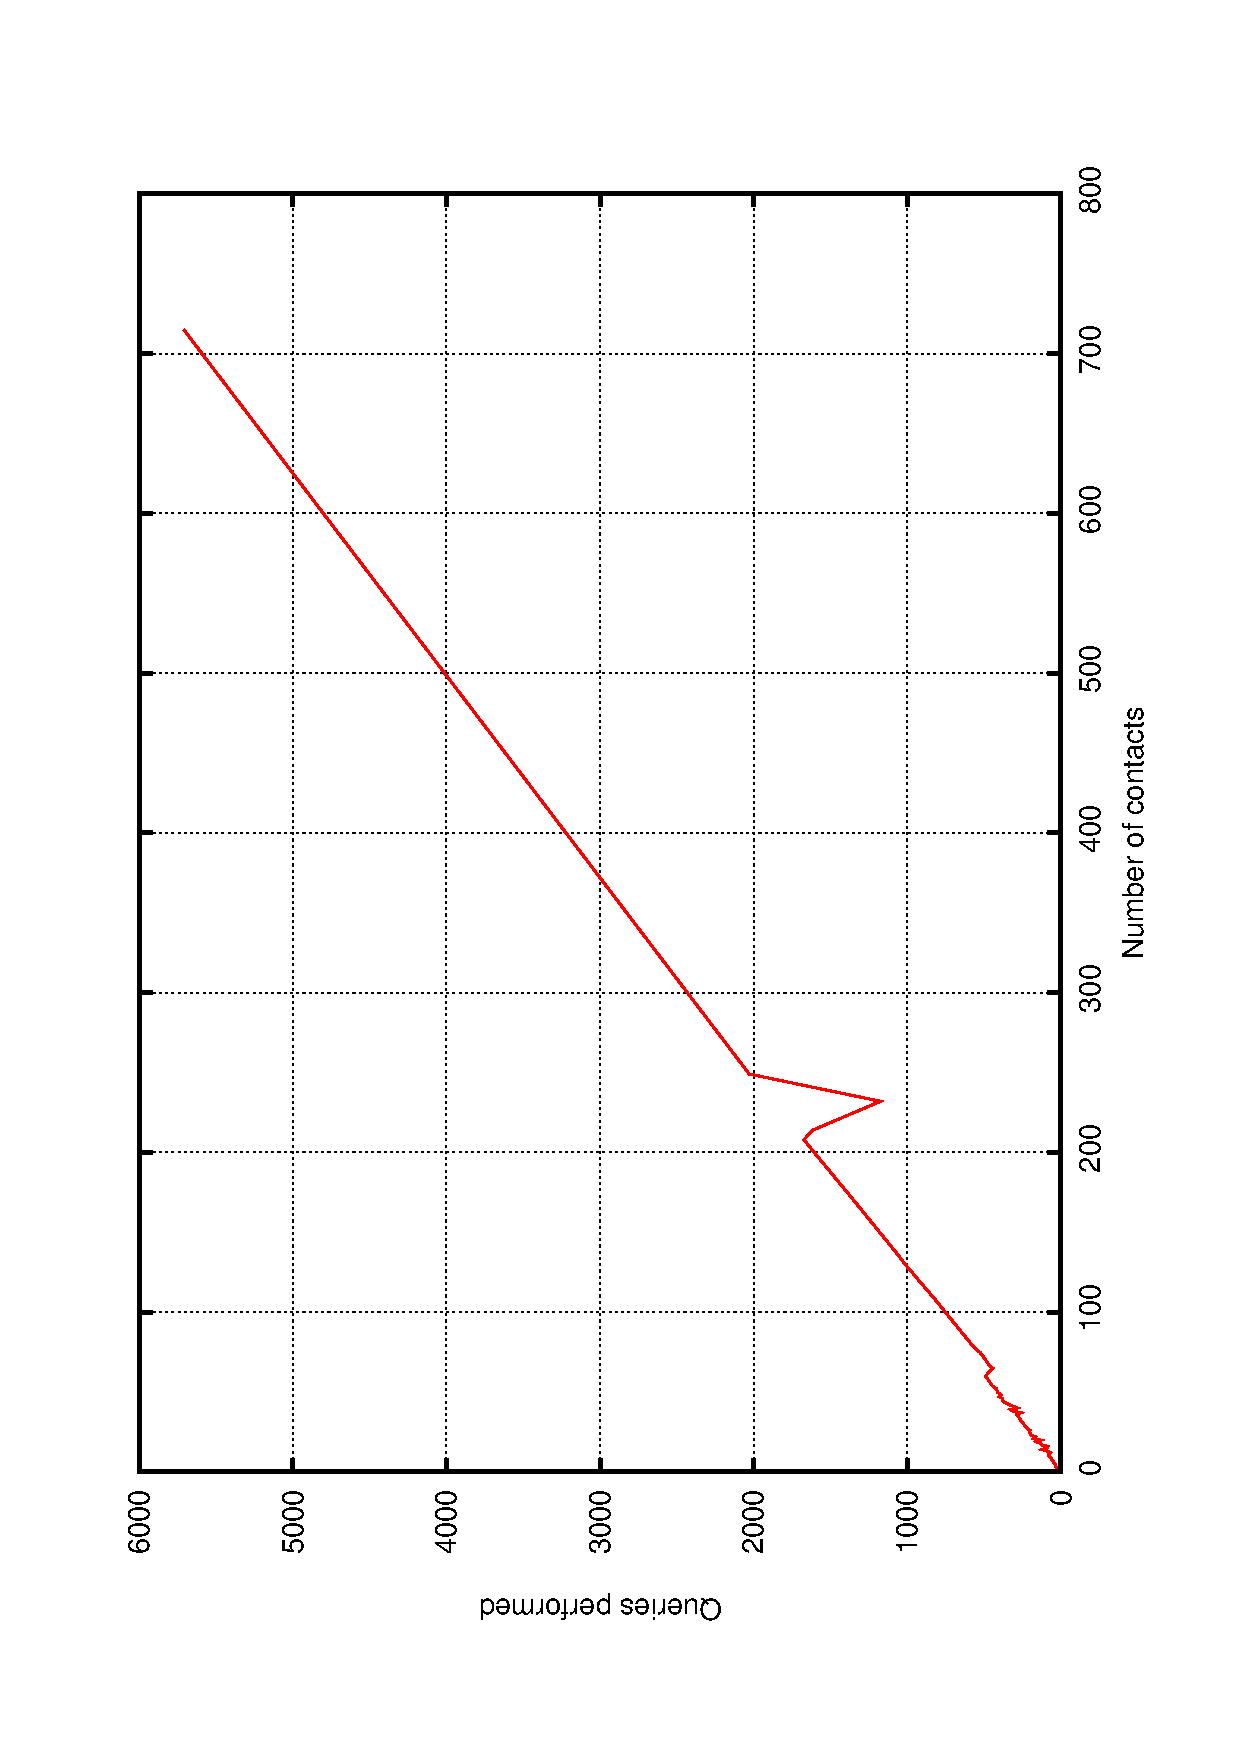
\includegraphics[width=155mm]{queries_per_contacts}
  \caption{Number of queries performed per number of contacts}
  \label{fig:queries_per_contacts}
\end{figure}

The implementation of the \textsc{Accountability} pattern to maintain the relationships between users was able to reduce the cost of the abovementioned task to $O(1)$: only 11 queries are performed to fetch and identify an user contacts, regardless of the size of said contact list. This means that the platform is able to sustain a considerable growth without suffering serious impacts on the performance of seemingly trivial operations.

\ \\
\textbf{NOTE: should Big O notation be used to express operation costs (i.e. number of queries performed)?}








\section{Documents}\label{sec:fa_documents}

\subsection{Variability Requirements}\label{sec:fa_documents_variability_requirements}

The document editor present in \emph{escolinhas.pt} is one of the core components of the system and one of the used features of the platform. This being the case, and due to the constantly evolving nature (\textbf{FIXME: it's not the nature that constantly evolves, but the product}), it is also one of the most modified parts of the system. As it can be seen in Fig.~\ref{fig:documents_current}, this structure has to grow both in size and complexity every time a new type of block content is introduced --- represented by the gray entities in Fig.~\ref{fig:documents_current}. This means that whenever a new type of content is introduced in the system, which happens somewhat frequently --- from three types of blocks (\emph{Paragraphs}, \emph{Drawings} and \emph{ImageDocuments/Photos}) in September 2009 to seven in April/May 2010 --- it is necessary to setup a new \textsc{ActiveRecord} class (along with all the logic for versioning) and a new \textsc{Controller} to accept the requests necessary to create, edit or delete any of these entities. Despite working as intended, this workflow is not adequate to the constant evolution and prototyping the document editor is subjected to.

\begin{figure}[H]
  \centering
  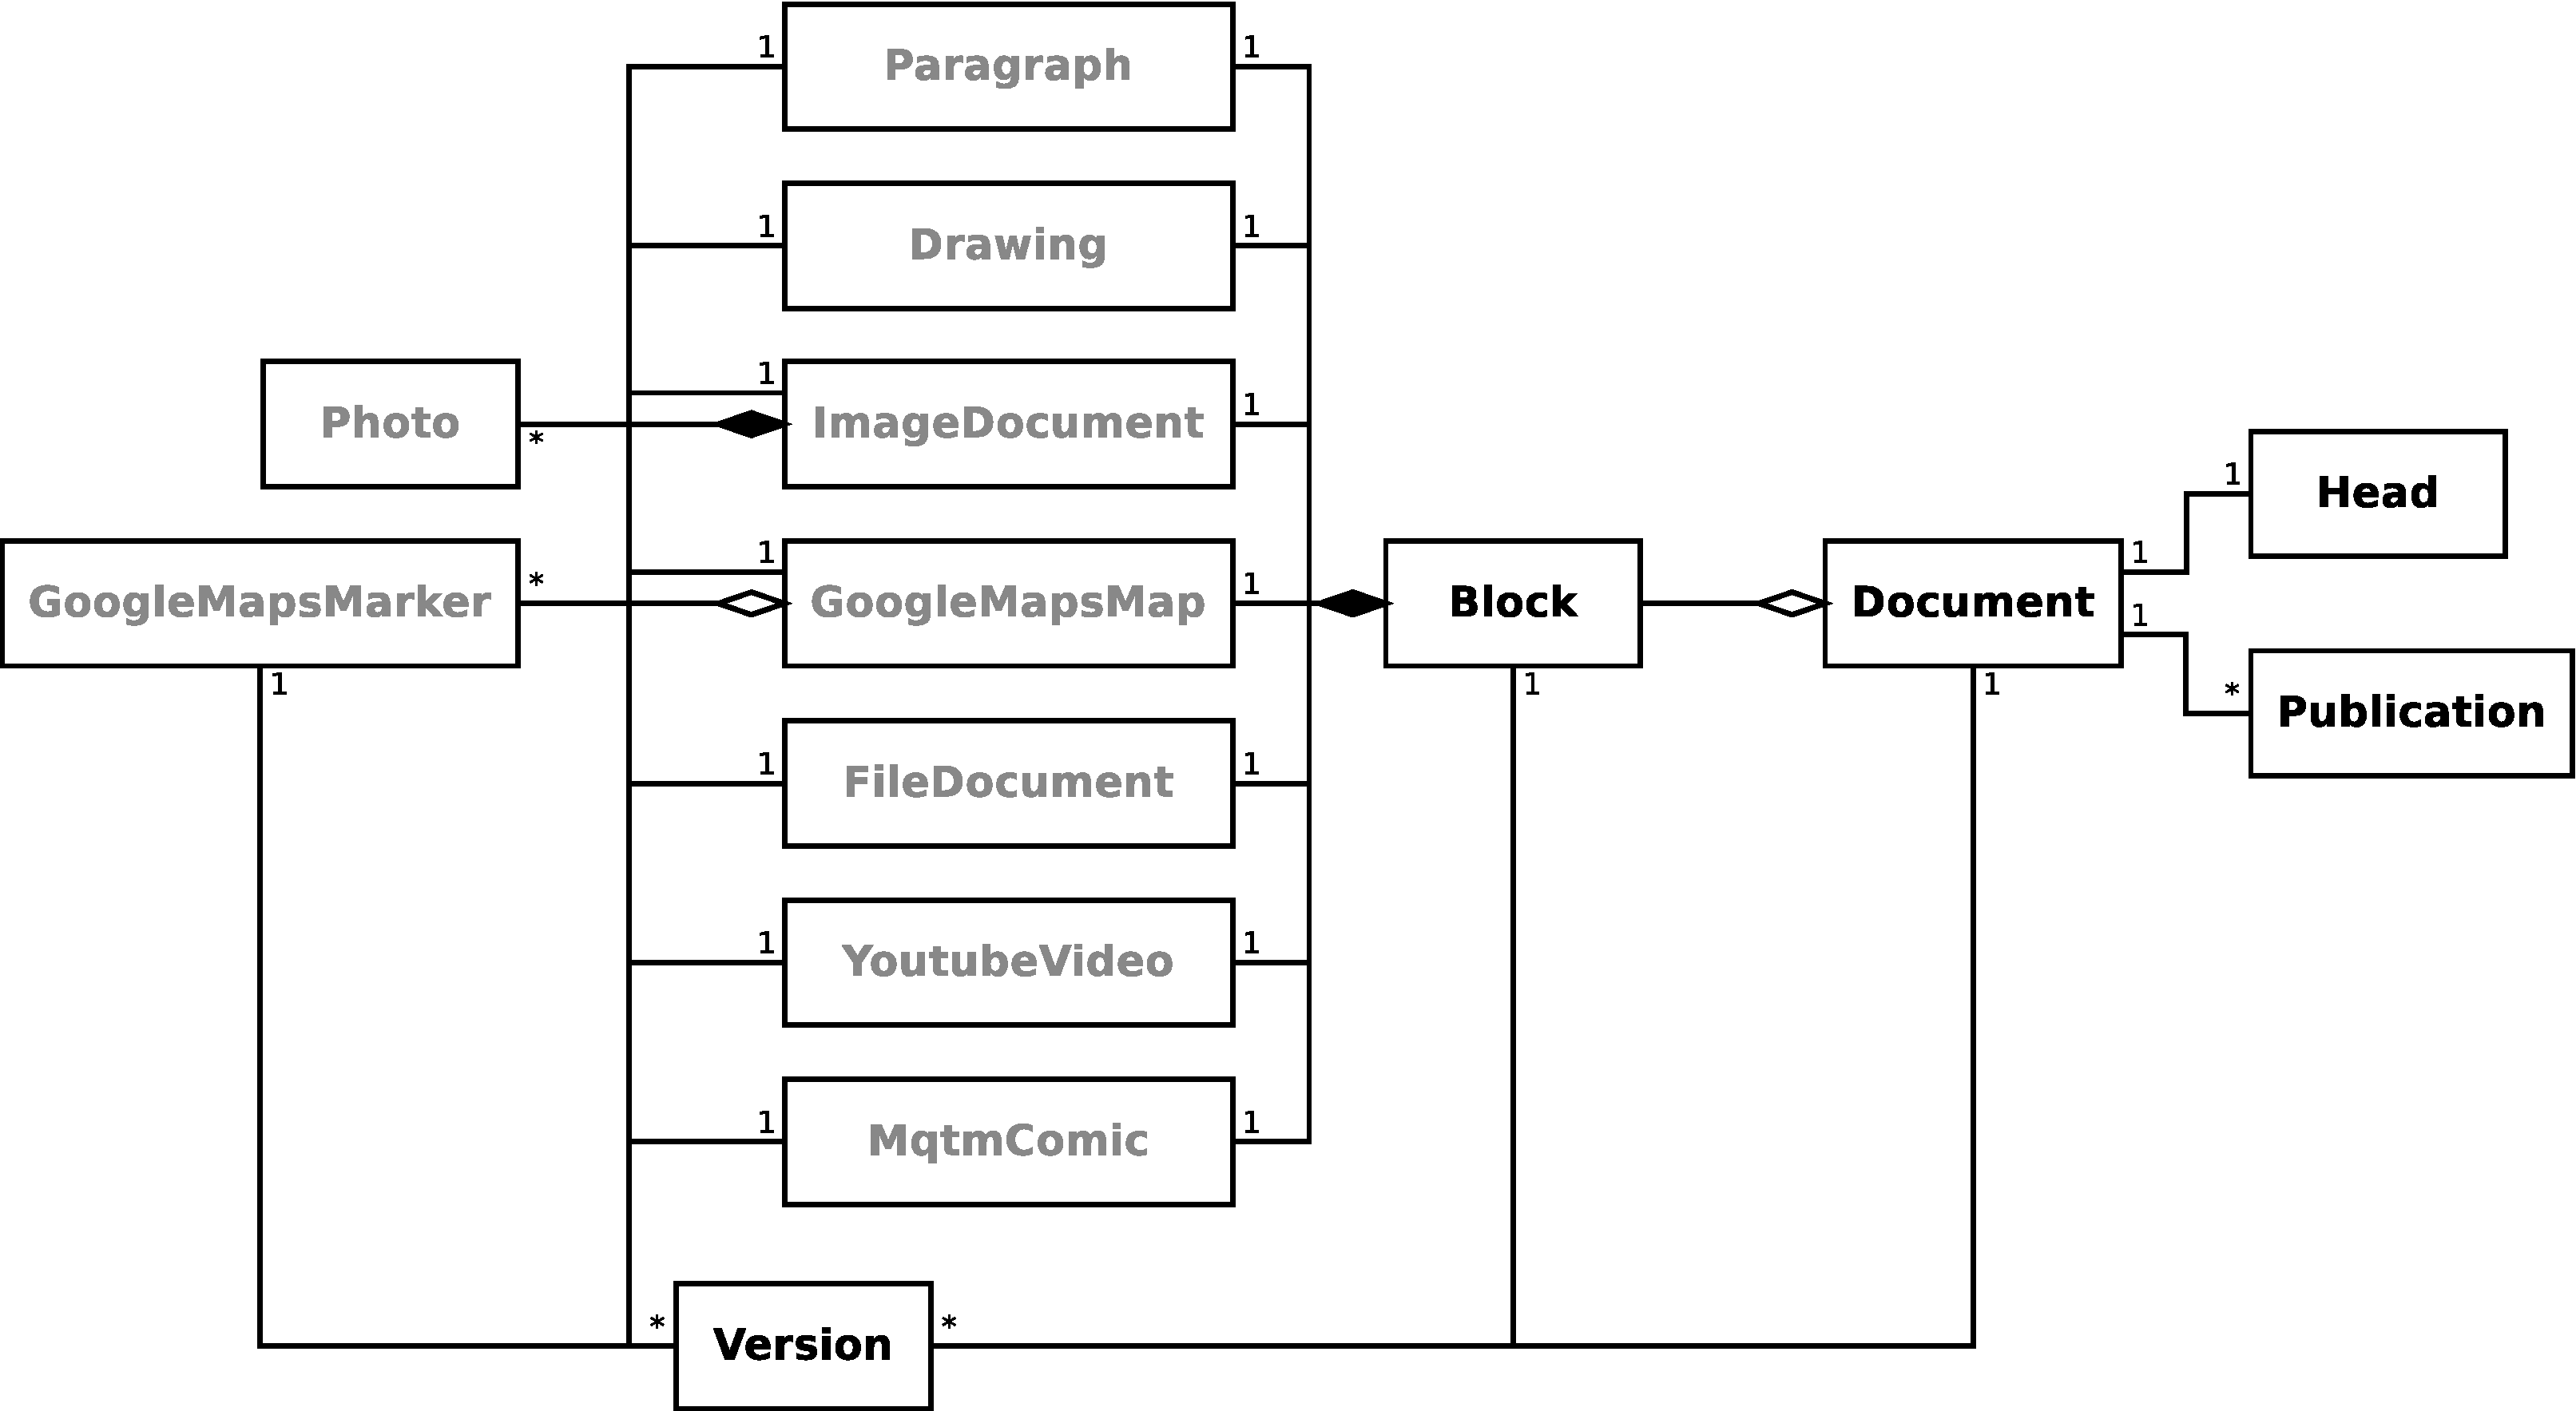
\includegraphics[width=165mm]{documents_current.pdf}
  \caption{Current Documents Model}
  \label{fig:documents_current}
\end{figure}

\subsection{Candidate Patterns}\label{sec:fa_documents_candidate_patterns}

\subsection{Chosen Patterns \& Rationale}\label{sec:fa_documents_chosen_patterns_rationale}

The pattern used is a composite design pattern as described in \cite{riehle_composite_patterns}, where various smaller design patterns work in tandem to create a more complex pattern:

\begin{itemize}
  \item \textsc{Memento} - used for versioning
  \item \textsc{Property} (simplified variant) - used for decoupling a \emph{Block content} from the database schema
  \item \textbf{INVESTIGATE: pattern 3} - the fact that a \emph{Publication} points to a specific \emph{Version} of a \emph{Document} may be a pattern --- it works as a \emph{tag} in a VCS (version control system) system such as git or SVN.
\end{itemize}

\begin{figure}[H]
  \centering
  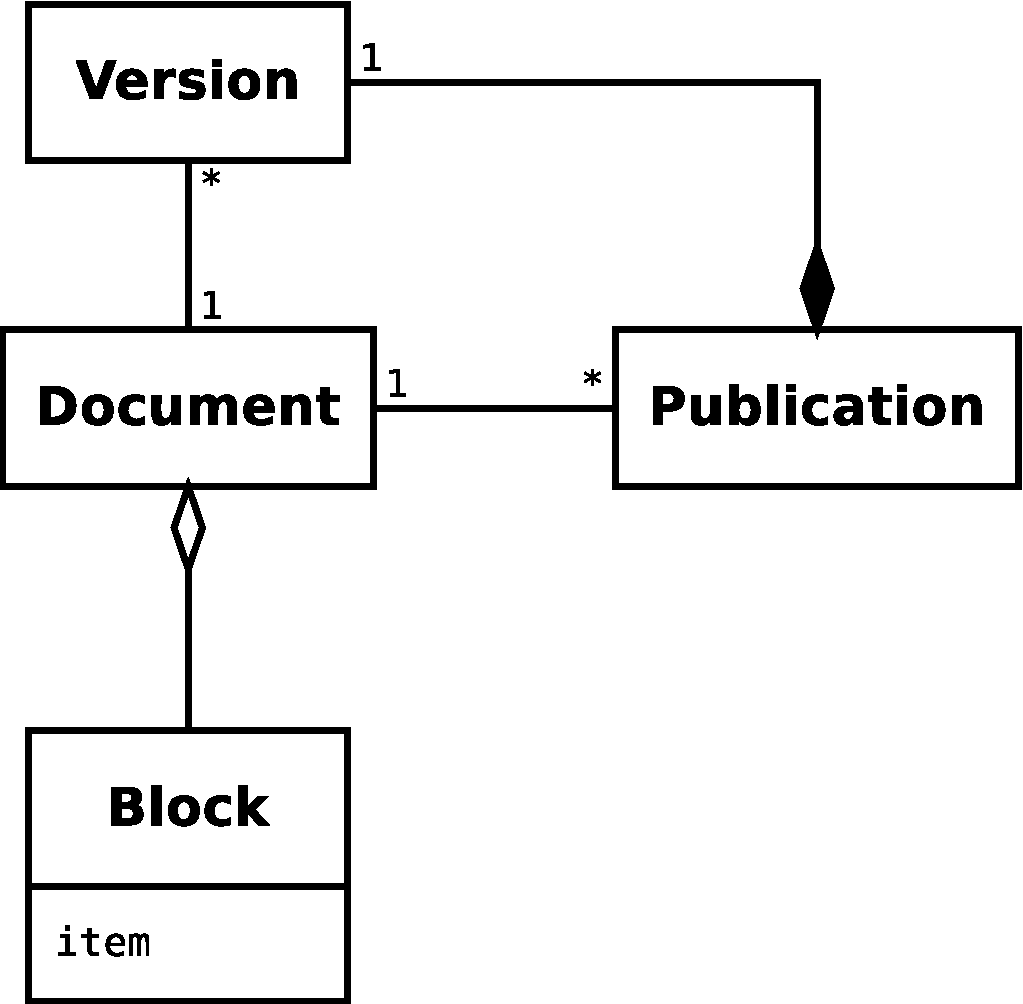
\includegraphics[width=75mm]{documents_conceptual.pdf}
  \caption{Conceptual Documents Model}
  \label{fig:documents_conceptual}
\end{figure}

The variant of the \textsc{Property} pattern implemented is simplified due to the highly dynamic nature of the Ruby language --- which means that, for this particular problem, it is able to build new types of objects or even create new class definitions in runtime, which allows discarding the \textsc{Property}--\textsc{PropertyType} pair (see \ref{sec:property_pattern}) in favour of a single entity, \emph{content}.

\subsection{Implementation}\label{sec:fa_documents_implementation}

The implementation of this composite pattern takes advantage of the highly dynamic nature of the Ruby language and the API provided by the \textsc{ActiveRecord} implementation of Rails.

\emph{Document}, \emph{Block}, \emph{Version} and \emph{Publication} are all AR objects, which means that, according to the AR pattern and the Rails framework conventions, each one of them is stored inside an SQL table, with a row for each one of the attributes. This structure provides the basic blueprint (as stated in \ref{sec:case-study_areas_document_editor}) for the documents to be produced by the editor --- it allows a title, an arbitrary number of orderable blocks, and a snapshot (version) of each modification. It also allows for publications, which essentially point to a specific version of a document.

There is nothing really remarkable about \emph{Blocks}, \emph{Documents} of even \emph{Publications} --- they are ordinary \textsc{ActiveRecord} objects, with associations to each other (as pictured in Fig.~\ref{fig:documents_conceptual}), and explaining how they work is outside of the scope of this study.

However, a \emph{Version} is a bit more complex than a simple AR object, in the sense that it contains a full representation of another AR object at a given point in time --- in this case, a \emph{Document}. This is achieved by serializing a \emph{Document} and all its associations (\emph{Blocks}) in the JSON format, which preserves all the necessary information needed to rebuild a specific \emph{Document} at whichever time that \emph{Version} refers to --- which means that a \emph{Version} effectively implements the \textsc{Memento} design pattern to keep a history of each \emph{Document}.

Finally, a \emph{Block} content possesses special properties that, together with AR, create a dynamic and variable foundation for the development of different types of content. As a \emph{Block} is simply a generic container for an arbitrary type of content, a \emph{Block} content can't be constrained to a single class or object type. The solution is to serialize the content inside the \emph{content} attribute of a \emph{Block}. This way, a \emph{Block} content is simply a string that represents a serialized object --- which can be de-serialized, accessed and modified at runtime. This means that, whichever a \emph{Block} content may be, the content itself is responsible for its representation and life cycle.

In order to further simplify and streamline the development, a \emph{DocumentItem} (super)class was created. This class serves as a staple for further specialization through inheritance, and handles cross-cutting concerns such as object initialization, default values and validations for each of these attribute's values. The need for a specific controller for each one of the different Block items has also been discarded in favour of a single controller, responsible for handling the user input regarding the modification of blocks and their content.

\subsection{Impact Analysis}\label{sec:fa_documents_impact_analysis}

The refactoring of the Document Editor infrastructure had two major points of impact: performance, and variability.


\subsubsection{Performance}

With the current foundation for the editor the number of queries grows linearly with the number of blocks that constitute a document, as it is necessary to perform a query for each one the items related to each one of the blocks. The usage of eager loading is limited due to the polymorphic nature of the blocks and each respective content, which is unknown \emph{a priori}.

From an universe of 3990 documents currently residing in the system (representative of all the documents present in the system as of November 23rd, 2010), the graph present in Fig.~\ref{fig:queries_per_blocks_in_document} shows a linear growth in the number of queries necessary to render a Document: the number of queries necessary are directly proportional to the number of blocks in a document with a 1:1 ratio. Just like in \ref{sec:fa_social_network_impact_analysis}, this represents a serious performance issue: as the most used feature in the \emph{escolinhas.pt} platform, a sustainable growth is very difficult to achieve if the database load increases linearly with the number of existent Documents.

\begin{figure}[H]
  \centering
  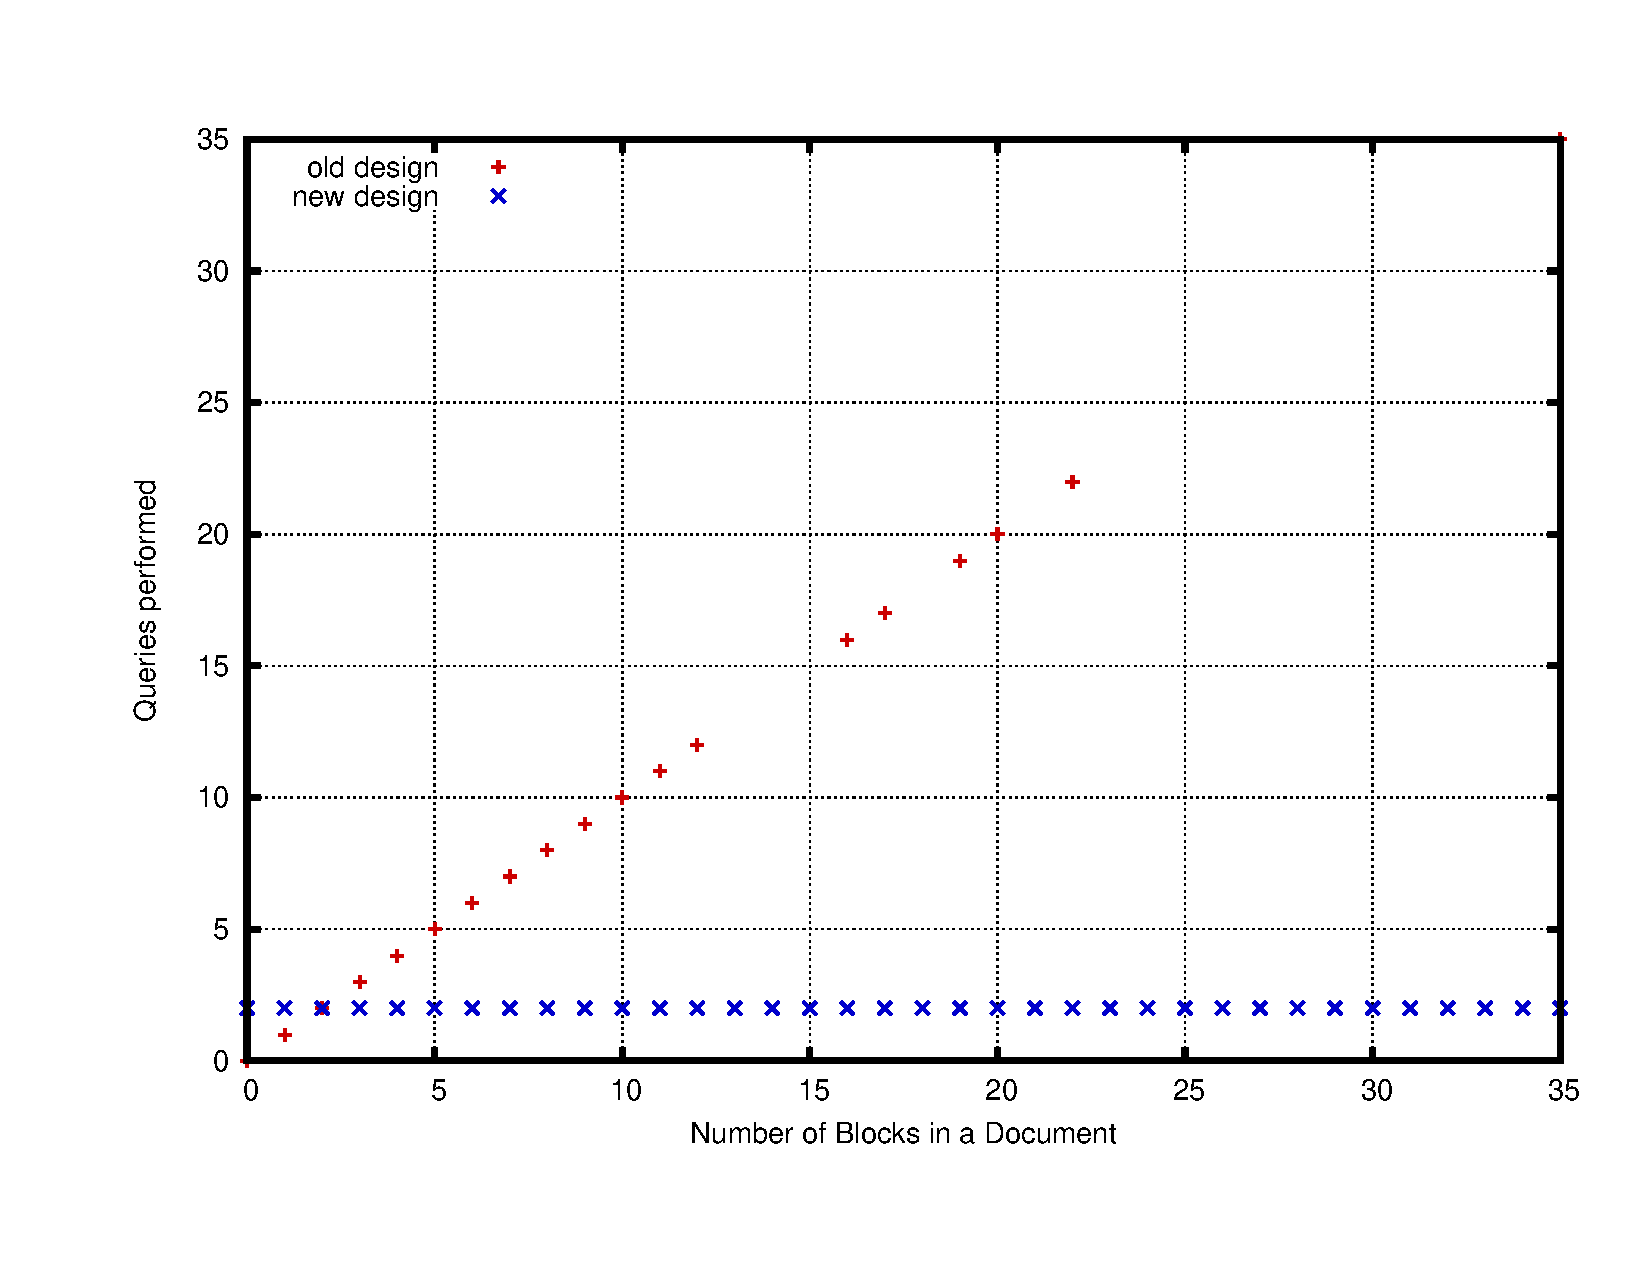
\includegraphics[width=145mm]{document_queries}
  \caption{Number of queries performed per number of Blocks in a single Document}
  \label{fig:queries_per_blocks_in_document}
\end{figure}

The introduction of the model described in \ref{sec:fa_documents_chosen_patterns_rationale} makes the number of queries necessary to display a \emph{Document} to be constant (only 2 queries are performed), as only the Blocks and the Document itself are AR objects --- as the item that constitutes a Block is an integral part of a Block, no queries are necessary to fetch it.

\subsubsection{Variability}

With the introduction of this model, the work necessary to create new types of blocks has been greatly reduced. This allows for much shorter prototyping and testing iteration times --- no database schemas or migrations to worry about, allowing the developers to focus on the details of the model rather than implementation details --- which ultimately leads to a higher degree of variability.











\section{Conclusions}\label{sec:approach_results_conclusions}

This chapter detailed how the study of the current design of the platform was conducted, and the tools used to do so. It described how the data gathered from that study was used to identify what the main problems within the platform were, and how they could be solved. It also described a vast set of applicable design patterns and how this set was reduced to choose the patterns that best solved the problem at hand. Finally, this chapter details the impact regarding the usage of each chosen pattern in terms of variability and performance.



